  
\section{Implementasi Antarmuka / \textit{User Interface}}
	
    \subsection{Antarmuka Registrasi}
    
    Penjelasan otorisasi terhadap antarmuka A, link yang tersedia dalam antarmuka A, dan penjelasan \textit{exception} jika terjadi masalah baik otorisasi ataupun autentikasi saat mengakses antarmuka ini.
  
      \begin{figure}[H]
        \centering
        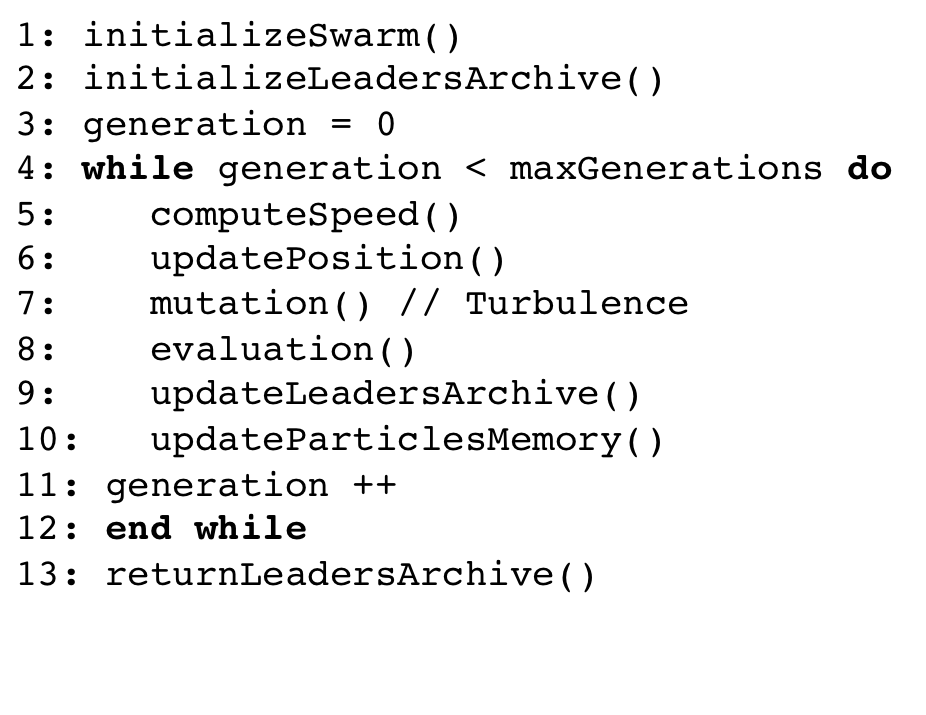
\includegraphics[width=\linewidth]{images/bab4/smpso_code.png}
        \caption{ Pseudocode Controller untuk Menampilkan Antarmuka A }
        \label{pdm}
      \end{figure}
      
    \subsection{Antarmuka Halaman B}
    Penjelasan otorisasi terhadap antarmuka B, link yang tersedia dalam antarmuka B, dan penjelasan \textit{exception} jika terjadi masalah baik otorisasi ataupun autentikasi saat mengakses antarmuka ini.
  
      \begin{figure}[H]
        \centering
        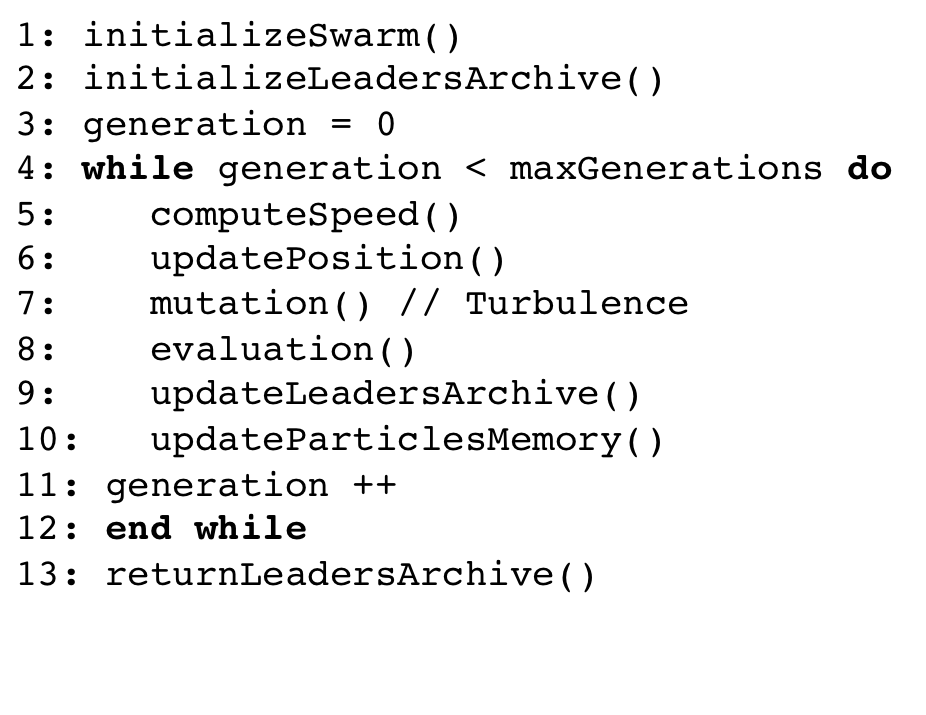
\includegraphics[width=\linewidth]{images/bab4/smpso_code.png}
        \caption{ Pseudocode Controller untuk Menampilkan Antarmuka B }
        \label{pdm}
      \end{figure}